% Drawn by docs/cicm/figures.mjs on 2026-10-21 from lean/Grothendieck/*.lean at HEAD
% and the parts of docs/lean/article.tex. Do not edit by hand.
\begin{figure}[t]\centering
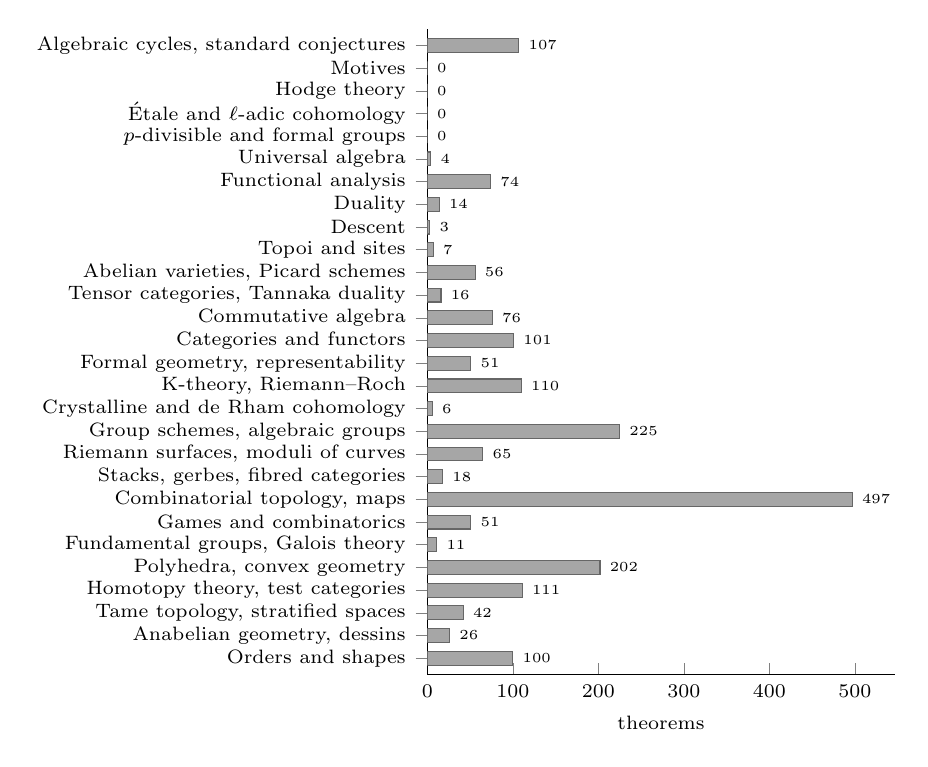
\begin{tikzpicture}
\begin{axis}[xbar, y=8.2pt, bar width=5pt, width=0.62\textwidth,
  xmin=0, enlarge y limits={abs=6pt}, xlabel={theorems}, xlabel style={font=\scriptsize},
  symbolic y coords={{Orders and shapes},{Anabelian geometry, dessins},{Tame topology, stratified spaces},{Homotopy theory, test categories},{Polyhedra, convex geometry},{Fundamental groups, Galois theory},{Games and combinatorics},{Combinatorial topology, maps},{Stacks, gerbes, fibred categories},{Riemann surfaces, moduli of curves},{Group schemes, algebraic groups},{Crystalline and de Rham cohomology},{K-theory, Riemann--Roch},{Formal geometry, representability},{Categories and functors},{Commutative algebra},{Tensor categories, Tannaka duality},{Abelian varieties, Picard schemes},{Topoi and sites},{Descent},{Duality},{Functional analysis},{Universal algebra},{$p$-divisible and formal groups},{Étale and $\ell$-adic cohomology},{Hodge theory},{Motives},{Algebraic cycles, standard conjectures}}, ytick=data,
  yticklabel style={font=\scriptsize}, xticklabel style={font=\scriptsize},
  nodes near coords, nodes near coords style={font=\tiny},
  axis x line*=bottom, axis y line*=left, every axis plot/.append style={fill=black!35, draw=black!60}]
\addplot[fill=black!35, draw=black!60] coordinates {(100,{Orders and shapes}) (26,{Anabelian geometry, dessins}) (42,{Tame topology, stratified spaces}) (111,{Homotopy theory, test categories}) (202,{Polyhedra, convex geometry}) (11,{Fundamental groups, Galois theory}) (51,{Games and combinatorics}) (497,{Combinatorial topology, maps}) (18,{Stacks, gerbes, fibred categories}) (65,{Riemann surfaces, moduli of curves}) (225,{Group schemes, algebraic groups}) (6,{Crystalline and de Rham cohomology}) (110,{K-theory, Riemann--Roch}) (51,{Formal geometry, representability}) (101,{Categories and functors}) (76,{Commutative algebra}) (16,{Tensor categories, Tannaka duality}) (56,{Abelian varieties, Picard schemes}) (7,{Topoi and sites}) (3,{Descent}) (14,{Duality}) (74,{Functional analysis}) (4,{Universal algebra}) (0,{$p$-divisible and formal groups}) (0,{Étale and $\ell$-adic cohomology}) (0,{Hodge theory}) (0,{Motives}) (107,{Algebraic cycles, standard conjectures})};
\end{axis}
\end{tikzpicture}
\caption{Lean theorems per theme, the themes being the 28 parts of the written-out appendix in their order (1973 of the 1973 theorems at HEAD; every file belongs to a part). The 4 parts at zero hold only statements left unproved. Drawn by \texttt{docs/cicm/figures.mjs} on 2026-10-21.}\label{fig:themes}
\end{figure}
